\newpage
\def\thoigian{90}%--Thời gian
\de{Đề số 2}{Chương I. Mệnh đề và Tập hợp}


% \everymath{\color{blue}}
\begin{center}
	\textbf{PHẦN 1 - CÂU TRẮC NGHIỆM BỐN PHƯƠNG ÁN}
\end{center}
\Opensolutionfile{ans}[ans/ans-TN-ONTAPCHUONG-DE1]
\begin{ex}%[0D1N1-1]%[Dự án đề kiểm tra Toán 10 GHKI NH23-24- VU Ngoc Hao]%[THPT Lê Quý Đôn - Ninh Thuận]
	Trong các câu sau, câu nào là mệnh đề chứa biến?
	\choice
	{$18$ chia hết cho $9$}
	{Hãy tìm các giá trị của $x$ và $y$ để $x+y=10$}
	{Có phải $x^2\ge 0$ với mọi $x$ thuộc $\mathbb{R}$ không?}
	{\True $3n$ chia hết cho $9$}
	\loigiai{
		Mệnh đề chứa biến là \lq\lq$3n$ chia hết cho $9$\rq\rq.
	}
\end{ex}

\begin{ex}%[0D1N1-5]%[Dự án đề kiểm tra Toán 10 GHKI NH23-24- VU Ngoc Hao]%[THPT Lê Quý Đôn - Ninh Thuận]
	Hãy phát biểu mệnh đề: \lq\lq $\exists n\in \mathbb{Z},\left| n\right|\le n$\rq\rq.
	\choice
	{\True Tồn tại số nguyên để nó không bé hơn trị tuyệt đối của nó}
	{ Tồn tại số tự nhiên để trị tuyệt đối của nó bé hơn hoặc bằng nó}
	{Trị tuyệt đối của mọi số nguyên đều bé hơn chính nó}
	{Tồn tại số nguyên để trị tuyệt đối của nó bé hơn chính nó}
	\loigiai{
		Tồn tại số nguyên để nó không bé hơn trị tuyệt đối của nó.
	}
\end{ex}

\begin{ex}%[0D1N1-4]%[Dự án đề kiểm tra Toán 10 GHKI NH23-24- VU Ngoc Hao]%[THPT Lê Quý Đôn - Ninh Thuận]
	Cho mệnh đề $P:$ \lq\lq Nếu hai tam giác đồng dạng và có một cạnh bằng nhau thì chúng bằng nhau\rq\rq. Mệnh đề đảo của mệnh đề $P$ là
	\choice
	{\True \lq\lq Nếu hai tam giác bằng nhau thì chúng đồng dạng và có một cạnh bằng nhau\rq\rq}
	{\lq\lq Hai tam giác đồng dạng và có một cạnh bằng nhau khi và chỉ khi chúng bằng nhau\rq\rq}
	{\lq\lq Nếu hai tam giác bằng nhau thì chúng có một cạnh bằng nhau\rq\rq}
	{\lq\lq Nếu hai tam giác bằng nhau thì chúng đồng dạng\rq\rq}
	\loigiai{Mệnh đề đảo của mệnh đề $P$ là \lq\lq Nếu hai tam giác bằng nhau thì chúng đồng dạng và có một cạnh bằng nhau\rq\rq.
	}
\end{ex}

\begin{ex}%[0D1N1-1]%[Dự án đề kiểm tra Toán 10 GHKI NH23-24- VU Ngoc Hao]%[THPT Lê Quý Đôn - Ninh Thuận]
	Trong các phát biểu sau, phát biểu nào là mệnh đề đúng?
	\choice
	{\True Số $5$ là số hữu tỷ}
	{$\pi $ là số tự nhiên}
	{Hình chữ nhật có hai đường chéo vuông góc}
	{Tam giác có một góc bằng $60^\circ$ là tam giác đều}
	\loigiai{
		Mệnh đề đúng là \lq\lq	Số $5$ là số hữu tỷ\rq\rq.
	}
\end{ex}
%Câu 5
\begin{ex}%[Dự án đề kiểm tra Toán 10 HKI NH23-24 - VU Ngoc Hao]%[THPT chuyên Lê Quý Đôn - Ninh Thuận]%[0D1N2-2]
	\immini{Cho hai tập hợp $A$ và $B$. Được biểu diễn bằng biểu đồ như hình bên. Khẳng định nào sau đây đúng?
		\choice
		{$B\subset A$}
		{$A=B$}
		{$A\cap B=\varnothing $}
		{\True $A\subset B$}}{
		\begin{tikzpicture}[scale=.6,thick,rotate=-99]
			\colorlet{MauNet}{black}
			\def\ElipA{(0,0) ellipse (2cm and 3cm)}
			\def\ElipB{(0.7,0.7) ellipse (0.7cm and 1.4cm)}
			\draw[MauNet,pattern=vertical lines,pattern color=white] \ElipA;
			\draw[MauNet,fill=white] \ElipB node[black]{$A$};
			\path[MauNet]\ElipA node[above left]{$B$};
			\draw[MauNet] (current bounding box.north) node[black,anchor=south] {};
		\end{tikzpicture}
	}
	\loigiai{
	Khẳng định đúng là \True $A\subset B$.
	}
\end{ex}

\begin{ex}%[0D1N3-1]%[Dự án đề kiểm tra Toán 10 GHKI NH23-24- VU Ngoc Hao]%[THPT Lê Quý Đôn - Ninh Thuận]
	\immini{Cho các tập hợp $A,B$ được minh hoạ bằng biểu đồ Ven như hình vẽ. Phần gạch sọc trong hình là biểu diễn của tập hợp nào sau đây?
		\choice
		{$A\cap B$}
		{$A\setminus B$}
		{$\mathrm{C}_BA$}
		{\True $A\cup B$}}{\begin{tikzpicture}[thick, scale=.8]
			\def\a{1.3}\def\r{2}
			\path (0:\a) coordinate (A) (180:\a) coordinate (B);
			\fill[pattern=north west lines]
			(B) circle (\r cm) 
			(A) circle (\r cm);
			\foreach \x in {A,B} \draw (\x) circle (\r cm);
			\node[] at (A) {$ B $};
			\node[] at (B) {$ A $};
	\end{tikzpicture}}
	\loigiai{Phần gạch sọc trong hình là biểu diễn của tập hợp $A\cup B$.
	}
\end{ex}
\begin{ex}%[0D1N3-4]%[Dự án đề kiểm tra Toán 10 GHKI NH24-25-ĐÀO HOÀNG VŨ]%[THPT TÂN BÌNH - Tp HCM]
	Cho $A$ và $B$ là hai tập hợp bất kì. Phần gạch sọc trong hình vẽ dưới đây là tập hợp nào sau đây
	\begin{center}
		\begin{tikzpicture}[line join=round, line cap=round,>=stealth,thick, scale=.5,rotate=30]
			
			\path (0,0) coordinate (O)
			;
			\draw[pattern=north west lines] (O) ellipse (5 cm and 3 cm);
			\draw[fill=white] (O) ellipse (3 cm and 2 cm);
			\path (-1,.5) node {$B$}
			(-4,-.5) node [fill=white] {$A$}
			;
			
		\end{tikzpicture}
	\end{center}
	\choice
	{$\mathrm{C}_B A$}
	{\True$\mathrm{C}_A B $}
	{$A\cup B$}
	{$A\cap B$}
	\loigiai{
		Phần gạch sọc là phần bù của $B$ trong $A$, kí hiệu $\mathrm{C}_A B$.
	}
\end{ex}
\begin{ex}%[0D1N2-2]%[Dự án đề kiểm tra Toán 10 GHKI NH24-25-ĐÀO HOÀNG VŨ]%[THPT TÂN BÌNH - Tp HCM]
	Cho tập hợp $A=\{0;1\}$. Tập hợp $A$ có bao nhiêu tập hợp con?
	\choice
	{$6$}
	{\True$4$}
	{$3$}
	{$2$}
	\loigiai{Số tập hợp con của tập hợp $A$ bằng $2^2=4$.}
\end{ex}
%Câu 9
\begin{ex}%[0D1N3-1]%[Dự án đề kiểm tra Toán 10 GHKI NH24-25-ĐÀO HOÀNG VŨ]%[THPT TÂN BÌNH - Tp HCM]
	Cho tập hợp $X=\{1;5\}$, $Y=\{1;3;5\}$. Tập $X\cap Y$ là tập hợp nào sau đây?
	\choice
	{$\{1\}$}
	{\True$\{1;5\}$}
	{$\{1;3;5\}$}
	{$\{1;3\}$}
	\loigiai{
		$X\cap Y=\{1;5\}$
	}
\end{ex}
\begin{ex}%[0D1H2-1]%[Dự án A KSCLDN 10-11 NH24-25- Phạm Văn Long]%[THPT Nguyễn Bỉnh Khiêm - Tp Hà Nội]
	Cho tập hợp $X=\left\{x \in \mathbb{Z} \mid x^2-2=0\right\}$. Mệnh đề nào sau đây là đúng?
	\choice
	{$X=\left\{-\sqrt{2}\right\}$}
	{$X=\left\{\sqrt{2}\right\}$}
	{\True $X=\varnothing$}
	{$X=\left\{-\sqrt{2}; \sqrt{2}\right\}$}
	\loigiai{
		Ta có $x^2-2=0\Rightarrow x=  \pm \sqrt{2}$. Vì $x \in \mathbb{Z}$ nên $X=\varnothing$.
	}
\end{ex}
\begin{ex}%[0D1N2-2]%[Dự án đề kiểm tra Toán 10 GHKI NH23-24- VU Ngoc Hao]%[THPT Lê Quý Đôn - Ninh Thuận]
	Cho tập $A=\left\{x\in{\mathbb{N}^{*}}\mid x\leq 5\right\}$, $B=\left\{0;1;2;3;4;5\right\}$. Phát biểu nào sau đây là đúng?
	\choice
	{$A=B$}
	{$A \in B$}
	{$B\subset A$}
	{\True $A\subset B$}
	\loigiai{ Tập $A=\left\{x\in{\mathbb{N}^{*}}\mid x\leq 5\right\}$. Tập $B=\left\{0;1;2;3;4;5\right\}$. Vậy  $A\subset B$.
	}
\end{ex}
\begin{ex}%[0D1H3-1]%[Dự án đề kiểm tra Toán 10 GHKI NH23-24- Phạm Hoài]%[THPT Lê Quý Đôn - Ninh Thuận]
	Cho tập hợp $B=(-\infty ; 4] \cup(2 ;+\infty) \cup[0 ; 3)$. Chọn khẳng định đúng trong các khẳng định sau
	\choice
	{$B=(-\infty ; 2)$}
	{$B=(0 ; 4]$}
	{$B=(0 ;+\infty)$}
	{\True $B=(-\infty ;+\infty)$}
	\loigiai{Ta có $B=(-\infty ; 4] \cup(2 ;+\infty) \cup[0 ; 3)=(-\infty;+\infty)$.
	}
\end{ex}
%\begin{ex}%[Dự án D - đợt 1 NH24-25 - VU Ngoc Hao]
%\end{ex}

\Closesolutionfile{ans}
%\begin{center}
%	\textbf{ĐÁP ÁN}
%	\inputansbox{10}{ans/ans}	
%\end{center}

\begin{center}
	\textbf{PHẦN 2 - CÂU TRẮC NGHIỆM ĐÚNG SAI}
\end{center}
\setcounter{ex}{0}
\Opensolutionfile{ans}[ans/answer-DS-ONTAPCHUONG-DE2]

\begin{ex}%[Đề kiểm tra GK1 THPT Nguyễn Bỉnh Khiêm - Cầu Giấy]%[Nguyễn Tấn Linh]%[0D1H1-4]
	Cho các câu sau:\\
	$P :$ \lq\lq Số tự nhiên $n$ có chữ số tận cùng bằng $5$\rq\rq.\\
	$Q :$ \lq\lq Số tự nhiên $n$ chia hết cho $5$\rq\rq.
	\choiceTF
	{\True Mệnh đề $P \Rightarrow Q$ được phát biểu là \lq\lq Nếu số tự nhiên $n$ có chữ số tận cùng bằng $5$ thì $n$ chia hết cho $5$\rq\rq}
	{\True Trong mệnh đề $P \Rightarrow Q$ thì $P$ là điều kiện đủ để có $Q$}
	{Mệnh đề $P \Rightarrow Q$ là một mệnh đề sai}
	{Trong mệnh đề $P \Rightarrow Q$ thì $Q$ là điều kiện cần và đủ để có $P$}
	\loigiai
	{
		\begin{itemchoice}
			\itemch Mệnh đề $P \Rightarrow Q$ được phát biểu là \lq\lq Nếu số tự nhiên $n$ có chữ số tận cùng bằng $5$ thì $n$ chia hết cho $5$\rq\rq .
			\itemch Trong mệnh đề $P \Rightarrow Q$ thì $P$ là điều kiện đủ để có $Q$.
			\itemch Số tự nhiên $n$ có chữ số tận cùng bằng $5$ thì số đó chia hết cho $5$.
			\itemch Trong mệnh đề $P \Rightarrow Q$ thì $Q$ là điều kiện cần để có $P$.
		\end{itemchoice}
	}
\end{ex}
\begin{ex}%[0D1V3-5]%[Lớp 10-HK1-THPT Chuyên Lê Quý Đôn - Ninh Thuận]%[Lê Hải Phụng]
	Lớp $10$A có $19$ học sinh tham gia câu lạc bộ cầu lông, $15$ học sinh tham gia câu lạc bộ bóng đá, $7$ học sinh tham gia cả hai câu lạc bộ cầu lông và bóng đá, $8$ học sinh không tham gia câu lạc bộ nào trong hai câu lạc bộ cầu lông và bóng đá. Gọi $A$ là tập các học sinh tham gia câu lạc bộ cầu lông, $B$ là tập các học sinh tham gia câu lạc bộ bóng đá.
	\choiceTF
	{\True Số phần tử của tập hợp $A\cap B$ là $7$}
	{\True Tập $A\cup B$ là tập tất cả các học sinh có tham gia ít nhất một trong hai câu lạc bộ cầu lông và bóng đá}
	{Số phần tử của tập hợp $A\setminus B$ là $4$}
	{\True Sĩ số lớp $10$A là $35$}
	\loigiai{Từ đề bài, ta có $n(A)=19$, $n(B)=15$, $n(A\cap B)=7$.
		\begin{itemchoice}
			\itemch  Số phần tử của tập hợp $A\cap B$ là $7$.
			\itemch  Tập $A\cup B$ là tập tất cả các học sinh có tham gia ít nhất một trong hai câu lạc bộ cầu lông và bóng đá.
			\itemch  Ta có $n(A\setminus B)=19-7=12$.
			\itemch  Số học sinh tham gia thể thao mà $n(A\cup B)=n(A)+n(B)-n(A\cap B)=19+15-7=27$.\\
			Do đó số học sinh lớp 10A là $n(A\cup B)+n\left(\overline{A \cup B}\right)=27+8=35$.
		\end{itemchoice}
	}
\end{ex}

\Closesolutionfile{ans}
%\inputansbox[2]{2}{ans/answer.tex}

\begin{center}
	\textbf{PHẦN 3 - CÂU TRẮC NGHIỆM TRẢ LỜI NGẮN}
\end{center}
\setcounter{ex}{0}
\Opensolutionfile{ans}[ans-KQ-ONTAPCHUONG-DE1]

% \begin{ex}%[0D1H3-1]%[Dự án đề kiểm tra Toán khối 10 HK1 NH24-25-Dot 5 - Khắc Thiên]%[THPT Chuyên Hùng Vương - Phú Thọ]
% 	Cho hai tập hợp $A=\left\{x \in \mathbb{R} \mid x^2-3x+2=0\right\}$; $B=\{n \in \mathbb{N} \mid n \leq 5\}$. Tìm số tập con của tập $A \cap B$.
% 	\shortans[]{4}
% 	\loigiai{Ta có $x^2-3x+2=0 \Rightarrow \hoac{&x=1\\&x=2}$. Khi đó $A=\{1;2\}$.\\
% 		Lại có $B=\{0;1;2;3;4;5\}$.\\
% 		Do đó, $A\cap B=\{1;2\}$.\\
% 		Vậy số tập con của tập $A \cap B$ là $2^2=4$ (tập hợp).
% 	}
% \end{ex}
\begin{ex}%[0D1H3-3] %[Dự án đề kiểm tra Toán khối 10 HK1 NH24-25-Dot 2 - Huỳnh Thanh Chí]%[Chuyên Bình Thuận-Bình Thuận]
	Cho $A=[m; m+1]$ và $B=(-\infty;-1) \cup[2;+\infty)$. Để $A\cap B=\varnothing$ thì $m \in[a; b)$. Tính $b-a$.
	\par\shortans[]{$2$}
	\loigiai{
		Để $A\cap B=\varnothing$ thì $\heva{& m\ge -1\\ & m+1<2}\Rightarrow -1\le m<1$.\\
		Khi đó $m\in [-1;1)$. Do đó $a=-1$, $b=1$.\\
		Vậy $b-a=1-(-1)=2$.
	}
\end{ex}

\begin{ex}%[Bùi Lợi- Dự án bộ đề 4 phần]%[0D1N2-3]	
	Cho tập $A=\left\{ x\in \mathbb{N} \mid x(2-x)(x^2-3x-4)=0 \right\}$. Hỏi tập $A$ có bao nhiêu tập con?
	\shortans{$8$}
	\loigiai{		
		Ta có $x(2-x)(x^2-3x-4)=0 \Rightarrow \hoac{
			& x=0 \in \mathbb{N} \\
			& x=2 \in \mathbb{N} \\
			& x=-1 \notin \mathbb{N} \\
			& x=4 \in \mathbb{N}.}$\\
		Vậy $A=\{0;2;4 \}$ nên $A$ có $8$ tập con là $\{0\}$; $\{2\}$; $\{ 4\}$; $\{2;4\}$; $\{0;4\}$; $\{0;2\}$; $\{0;2;4\}$; $\varnothing$.
	}
\end{ex}
\begin{ex}%[Bùi Lợi-Dự án bộ đề 4 phần]%[0D1V2-2]
	Cho hai tập hợp khác rỗng $A=(1;5)$ và $B=(m;4m-1) \neq \varnothing$, $m \in \mathbb{R}$. Có bao nhiêu giá trị nguyên của tham số $m$ để $B \subset A$.
	\par\shortans{$1$}
	\loigiai{
		Vẽ trục số thể hiện $B \subset A$.
		\begin{center}
			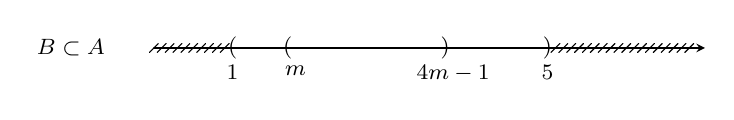
\begin{tikzpicture}[scale=1,>=stealth, font=\footnotesize, line join=round, line cap=round]
				\draw [-stealth] (0,0)--(7,0);
				\path (1,0) node{$($} (1,-0.1)node[below]{$1$} (-.5,0)node[left]{$B \subset A$};
				\path (5,0) node{$)$} (5,-0.1)node[below]{$5$};
				\path (1.7,0) node{$($} (1.8,-0.1)node[below]{$m$};
				\path (3.7,0) node{$)$} (3.8,-0.1)node[below]{$4m-1$};
				\foreach \x in{0,0.1,...,1} \draw (\x,0)--++(45:.08) (\x,0)--++(-135:.08);
				\foreach \x in{5.1,5.2,...,6.8} \draw (\x,0)--++(45:.08) (\x,0)--++(-135:.08);
			\end{tikzpicture}
		\end{center}
		Để $B \neq \varnothing $ thì $m<4 m-1 \Rightarrow m>\dfrac{1}{3}$. \quad $(1)$\\
		Và 
		$B\subset A 
		\Rightarrow \heva{&m \geq 1\\&4m-1\leq 5} 
		\Rightarrow 1 \leq m \leq \dfrac{3}{2}$. \quad $(2)$\\
		Từ $(1)$, $(2)$ suy ra $1 \leq m \leq \dfrac{3}{2}$.\\
		Vậy có $1$ giá trị nguyên của $m$ thì $B \subset A$.
	}
\end{ex}
\begin{ex}%[0D1V3-5]%[Dự án đề kiểm tra Toán khối 10 HK1 NH24-25-Dot 5 - Khắc Thiên]%[THPT Chuyên Hùng Vương - Phú Thọ]
	Lớp $10$A có $35$ học sinh. Trong đợt đăng kí câu lạc bộ thể dục đầu năm, mỗi học sinh đăng kí từ một đến ba câu lạc bộ gồm: bóng đá, cầu lông, đá cầu. Thống kê theo từng câu lạc bộ có: $20$ học sinh đăng kí câu lạc bộ bóng đá; $15$ học sinh đăng kí câu lạc bộ cầu lông; $9$ học sinh đăng kí câu lạc bộ đá cầu. Thống kê theo nhóm hai câu lạc bộ có: $4$ học sinh đăng kí câu lạc bộ bóng đá và cầu lông; $4$ học sinh đăng kí câu lạc bộ cầu lông và đá cầu; $3$ học sinh đăng kí câu lạc bộ đá cầu và bóng đá. Hỏi có bao nhiêu học sinh đăng kí cả ba câu lạc bộ?
	\par\shortans[oly]{$2$}
	\loigiai{
		Gọi $A$: tập hợp học sinh đăng ký bóng đá.\\
		Gọi $B$: tập hợp học sinh đăng ký cầu lông.\\
		Gọi $C$: tập hợp học sinh đăng ký đá cầu.\\
		Theo đề bài ta có \\
		$n(A)=20$ (học sinh đăng ký bóng đá).\\
		$n(B)=15$ (học sinh đăng ký cầu lông).\\
		$n(C)=9$ (học sinh đăng ký đá cầu).\\
		$n(A \cap B)=4$ (học sinh đăng ký cả bóng đá và cầu lông).\\
		$n(B \cap C)=4$ (học sinh đăng ký cà cầu lông và đá cầu).\\
		$n(C \cap A)=3$ (học sinh đăng ký cà đá cầu và bóng đá).\\
		Tổng số học sinh trong lớp $n(A \cup B \cup C)=35$.\\
		Chúng ta cần tìm số học sinh đăng ký cả $3$ câu lạc bộ, gọi số này là $x$.\\
		Theo công thức của số phần tử trong hợp của ba tập hợp, ta có
		\begin{eqnarray*}
			n(A \cup B \cup C)=n(A)+n(B)+n(C)-n(A \cap B)-n(B \cap C)-n(C \cap A)+n(A \cap B \cap C).
		\end{eqnarray*}
		Thay các giá trị đã biết vào công thức
		\begin{eqnarray*}
			35&=&20+15+9-4-4-3+x\\
			\Rightarrow 35&=&44-11+x\\
			\Rightarrow 35&=&33+x\\
			\Rightarrow x&=&35-33=2.
		\end{eqnarray*}
		Vậy có $2$ học sinh đăng ký cả $3$ câu lạc bộ.
	}
\end{ex}
\Closesolutionfile{ans}

\begin{center}
	\textbf{PHẦN 4 - TỰ LUẬN}
\end{center}
\setcounter{ex}{0}

\begin{ex}%[0D1V1-2]%[Dự án đề kiểm tra Toán 10 GHKI NH23-24- Phạm Hoài]%[THPT Lê Quý Đôn - Ninh Thuận]
	Xác định tính đúng, sai và lập mệnh đề phủ định của mệnh đề sau
	\lq \lq $ Q:\,  \forall x \in \mathbb{Z}, \, \dfrac{2 x^3-6 x^2+x-3}{2 x^2+1} \in \mathbb{Z}$\rq \rq.
	\loigiai{$\dfrac{2 x^3-6 x^2+x-3}{2 x^2+1}=\left(x-3\right)\left(x^2+1\right)$.\\
		Do đó $\forall x\in \mathbb{Z} $ thì $\dfrac{2 x^3-6 x^2+x-3}{2 x^2+1} \in \mathbb{Z}$.\\
		Vậy $Q$ là mệnh đề đúng.\\ 
		Gọi $\overline{Q}$ là mệnh đề phủ định của mệnh đề $Q$. Khi đó: $\overline{Q}:$ \lq \lq  $\exists x\in \mathbb{Z}, \dfrac{2 x^3-6 x^2+x-3}{2 x^2+1} \notin \mathbb{Z} $\rq \rq.
	}
\end{ex}

\begin{ex}%[0D12H-1]
	Xác định tập hợp $X$ biết $\{a, 1\} \subset X \subset \{a, b, 1, 2\}$.
\loigiai{
Ta có
\begin{itemize}
    \item Vì $\{a, 1\} \subset X$ nên tập hợp $X$ có chứa $2$ phần tử là $a$, $1$.
    \item Vì $X \subset \{a, b, 1, 2\}$ nên các phần tử của tập hợp $X$ có thể là $a$, $b$, $1$, $2$.
\end{itemize}
Suy ra, tập hợp $X$ có $2$ phần tử, $3$ phần tử hoặc $4$ phần tử.\\
Khi đó, tập hợp $X$ có thể là $\{a, 1\}$, $\{a, 1, 2\}$, $\{a, b, 1\}$, $\{a, b, 2\}$, $\{a, b, 1, 2\}$.
}
\end{ex}

\begin{ex}%[0D1H3-5]%[Dự án đề kiểm tra Toán 10 GKI NH24-25- Quan Ón]%[THPT Phạm Phú Thứ - Tp HCM]
	Trong đợt thi giải chạy ngắn cấp trường, lớp $10$B có $15$ học sinh đăng kí thi nội dung $100$ m, $10$ học sinh đăng kí thi nội dung $200$ m. Biết lớp $10$B có $40$ học sinh và có $18$ học sinh không đăng kí thi nội dung nào trong hai nội dung trên.
	\begin{enumerate}
		\item Lớp $10$B có bao nhiêu học sinh đăng kí ít nhất một trong hai nội dung trên?
		\item Lớp $10$B có bao nhiêu học sinh đăng kí cả hai nội dung trên?
	\end{enumerate}
	\loigiai{
		\immini{
			$\begin{aligned}[t]
				\text{Gọi } &A \text{ là tập hợp học sinh lớp $10$B đăng kí thi nội dung $100$ m,}\\
				&B \text{ là tập hợp học sinh lớp $10$B đăng kí thi nội dung $200$ m}.
			\end{aligned}$\\
			Theo đề bài, ta có $n(A) = 15$, $n(B) = 10$.
			\begin{enumerate}
				\item Số học sinh lớp $10$B đăng kí ít nhất một trong hai nội dung trên là
				$$ n(A\cup B) = 40 - 18 = 22 \textrm{ (học sinh).}$$
				\item Số học sinh lớp $10$B đăng kí cả hai nội dung trên là
				$$ n(A\cap B) = n(A) + n(B) - n(A\cup B) = 15 + 10 - 22 = 3 \textrm{ (học sinh).} $$
			\end{enumerate}
		}{
			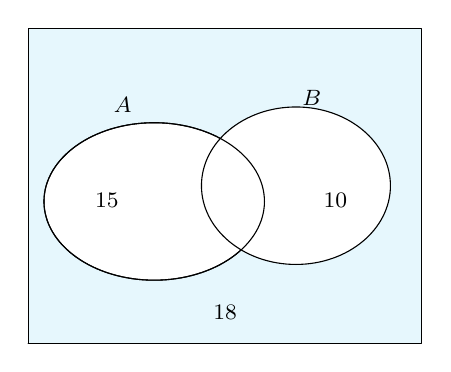
\begin{tikzpicture}[>=stealth,line join=round,line cap=round,font=\footnotesize,scale=1]
				\filldraw[fill = cyan!10] (0,0)--(5,0)--(5,4)--(0,4)--(0,0);
				\filldraw[fill = white] (1.6,1.8) ellipse (1.4cm and 1cm);
				\filldraw[fill = white] (3.4,2) ellipse (1.2cm and 1cm);
				\draw (1.6,1.8) ellipse (1.4cm and 1cm);
				\path 
				(1.2,2.8) node[above]{$A$}
				(3.6,2.9) node[above]{$B$}
				(1,1.6) node[above]{$15$}
				(3.9,1.6) node[above]{$10$}
				(2.5,0.6) node[below]{$18$}
				;
			\end{tikzpicture}
		}
	}
\end{ex}


